\chapter{Background}

%%%%%%%%%%%%%%%%%%%%%%
%        CMS
%%%%%%%%%%%%%%%%%%%%%%

\section{Compact Muon Solenoid (CMS) Detector}

The Compact Muon Solenoid (CMS) detector be designed for collect the collision and decaying data in forward and transverse of the beamline.
It has more resolution in the transverse direction from the equipment that has been designed to focus in transverse direction as the Figure \ref{fig:cms_structure}.
According to \cite{cms_design_report}, The detector itself consist of different sub-detector for their own purpose where the main components are

The Compact Muon Solenoid (CMS) detector be designed to collect the collision and decay-ing data in forward and transverse of the beamline.
It has more resolution in the transverse direction from the equipment that has been designed to focus in transverse direction as Figure \ref{fig:cms_online_system}.
According to \cite{cms_design_report}, The detector itself consists of different sub-detector for their own purpose where the main components are

\begin{figure}[h!]
    \centering
    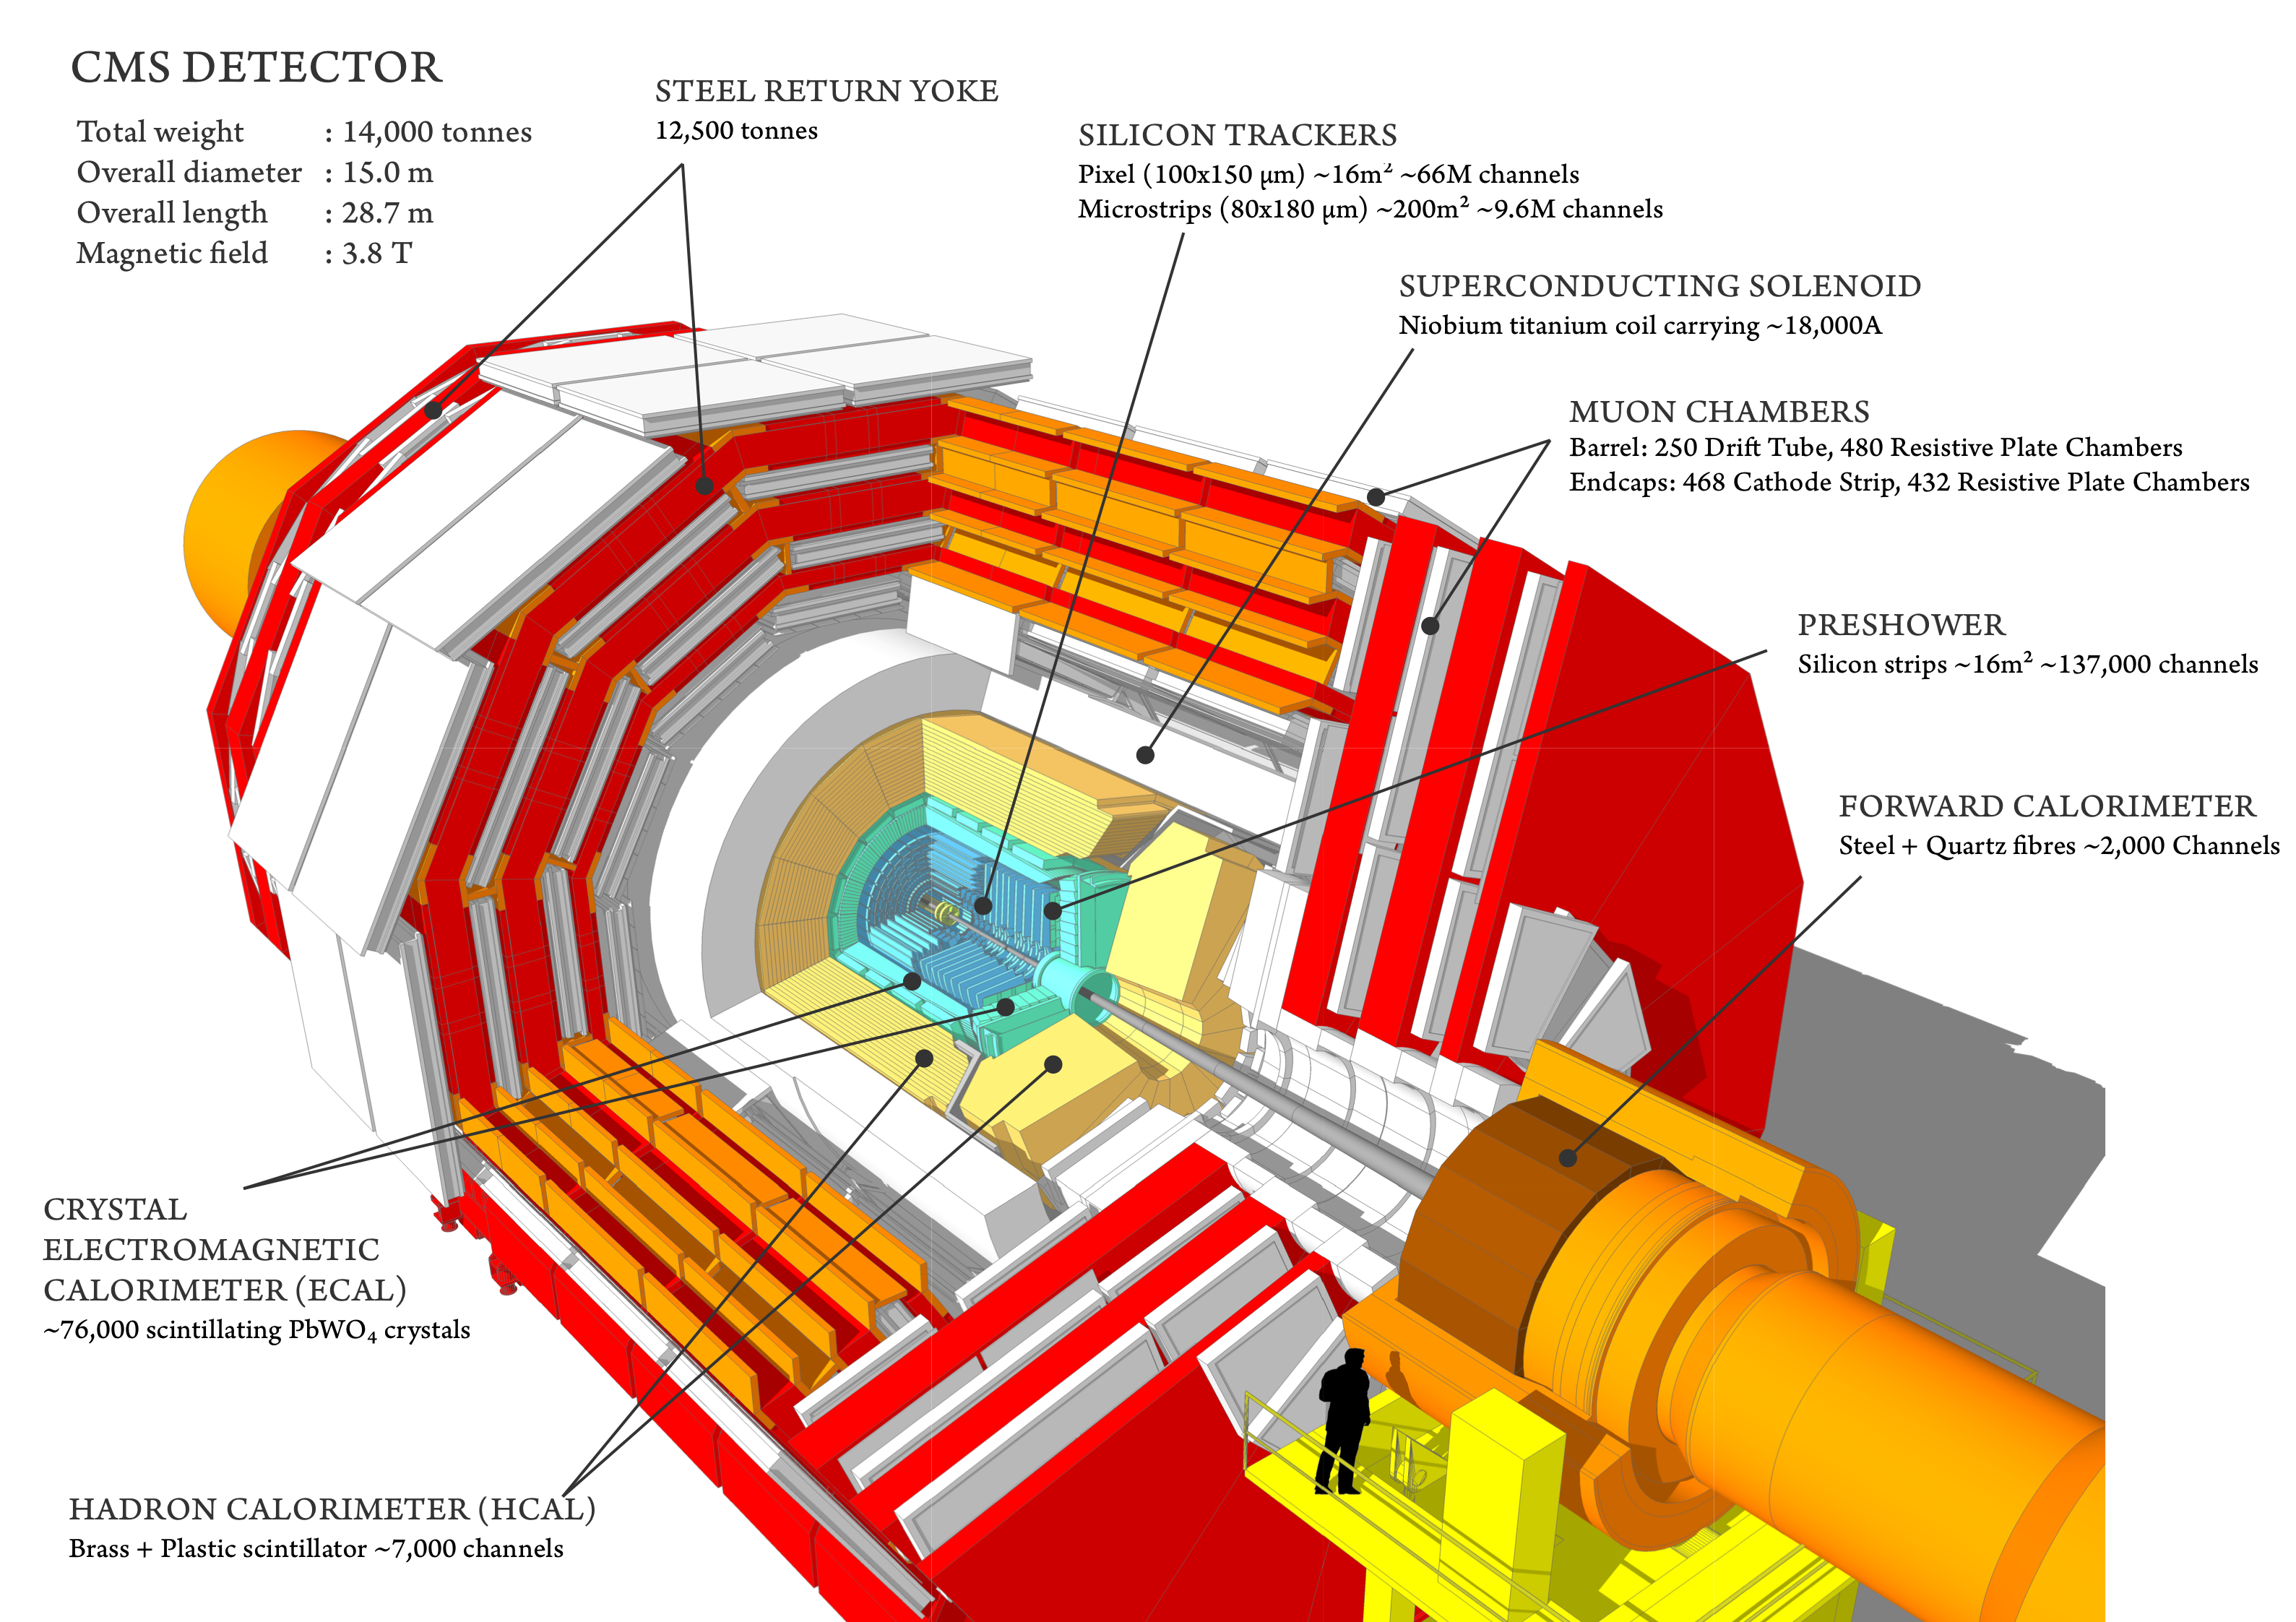
\includegraphics[width=0.8\textwidth]{images/cms_structure.png}
    \caption{Sectional view of the CMS detector. The LHC beams travel in opposite directions along the central axis of the CMS cylinder colliding in the middle of the CMS detector. Image retrieved from http://cms.web.cern.ch/news/cms-detector-design}
    \label{fig:cms_structure}
\end{figure}
\begin{enumerate}
    \item \textbf{Tracker} to trace the footprint of a charged particle by beginning at the hitting of the closest layer which is pixel detector and following by multiple layers of strip detector to gain more precision of particle tracks that correspond to momentum of the particle
    \item \textbf{Electromagnetic Calorimeter (ECAL)} measure the momentum of leptons (especially electron) and photon where the main interaction is electromagnetic interaction
    \item \textbf{Hadron Calorimeter (HCAL)} has been designed for measure the energy of hadronic particle where it also has QCD interaction rather than only electromagnatic
    \item \textbf{Superconducting Solenoid} for generate a nearly-uniform magnetic field inside of the cylindrical shape and charged particle turn their heading around where it propagate in the outside of this radius like a muon track in Figure \ref{fig:cms_slide}
    \item \textbf{Muon Detectors} is one of the most important sub-detector for measuring the muon momentum and the track of them by taking a footprint of tracking system into account to get more precise information
\end{enumerate}
\begin{figure}[h!]
    \centering
    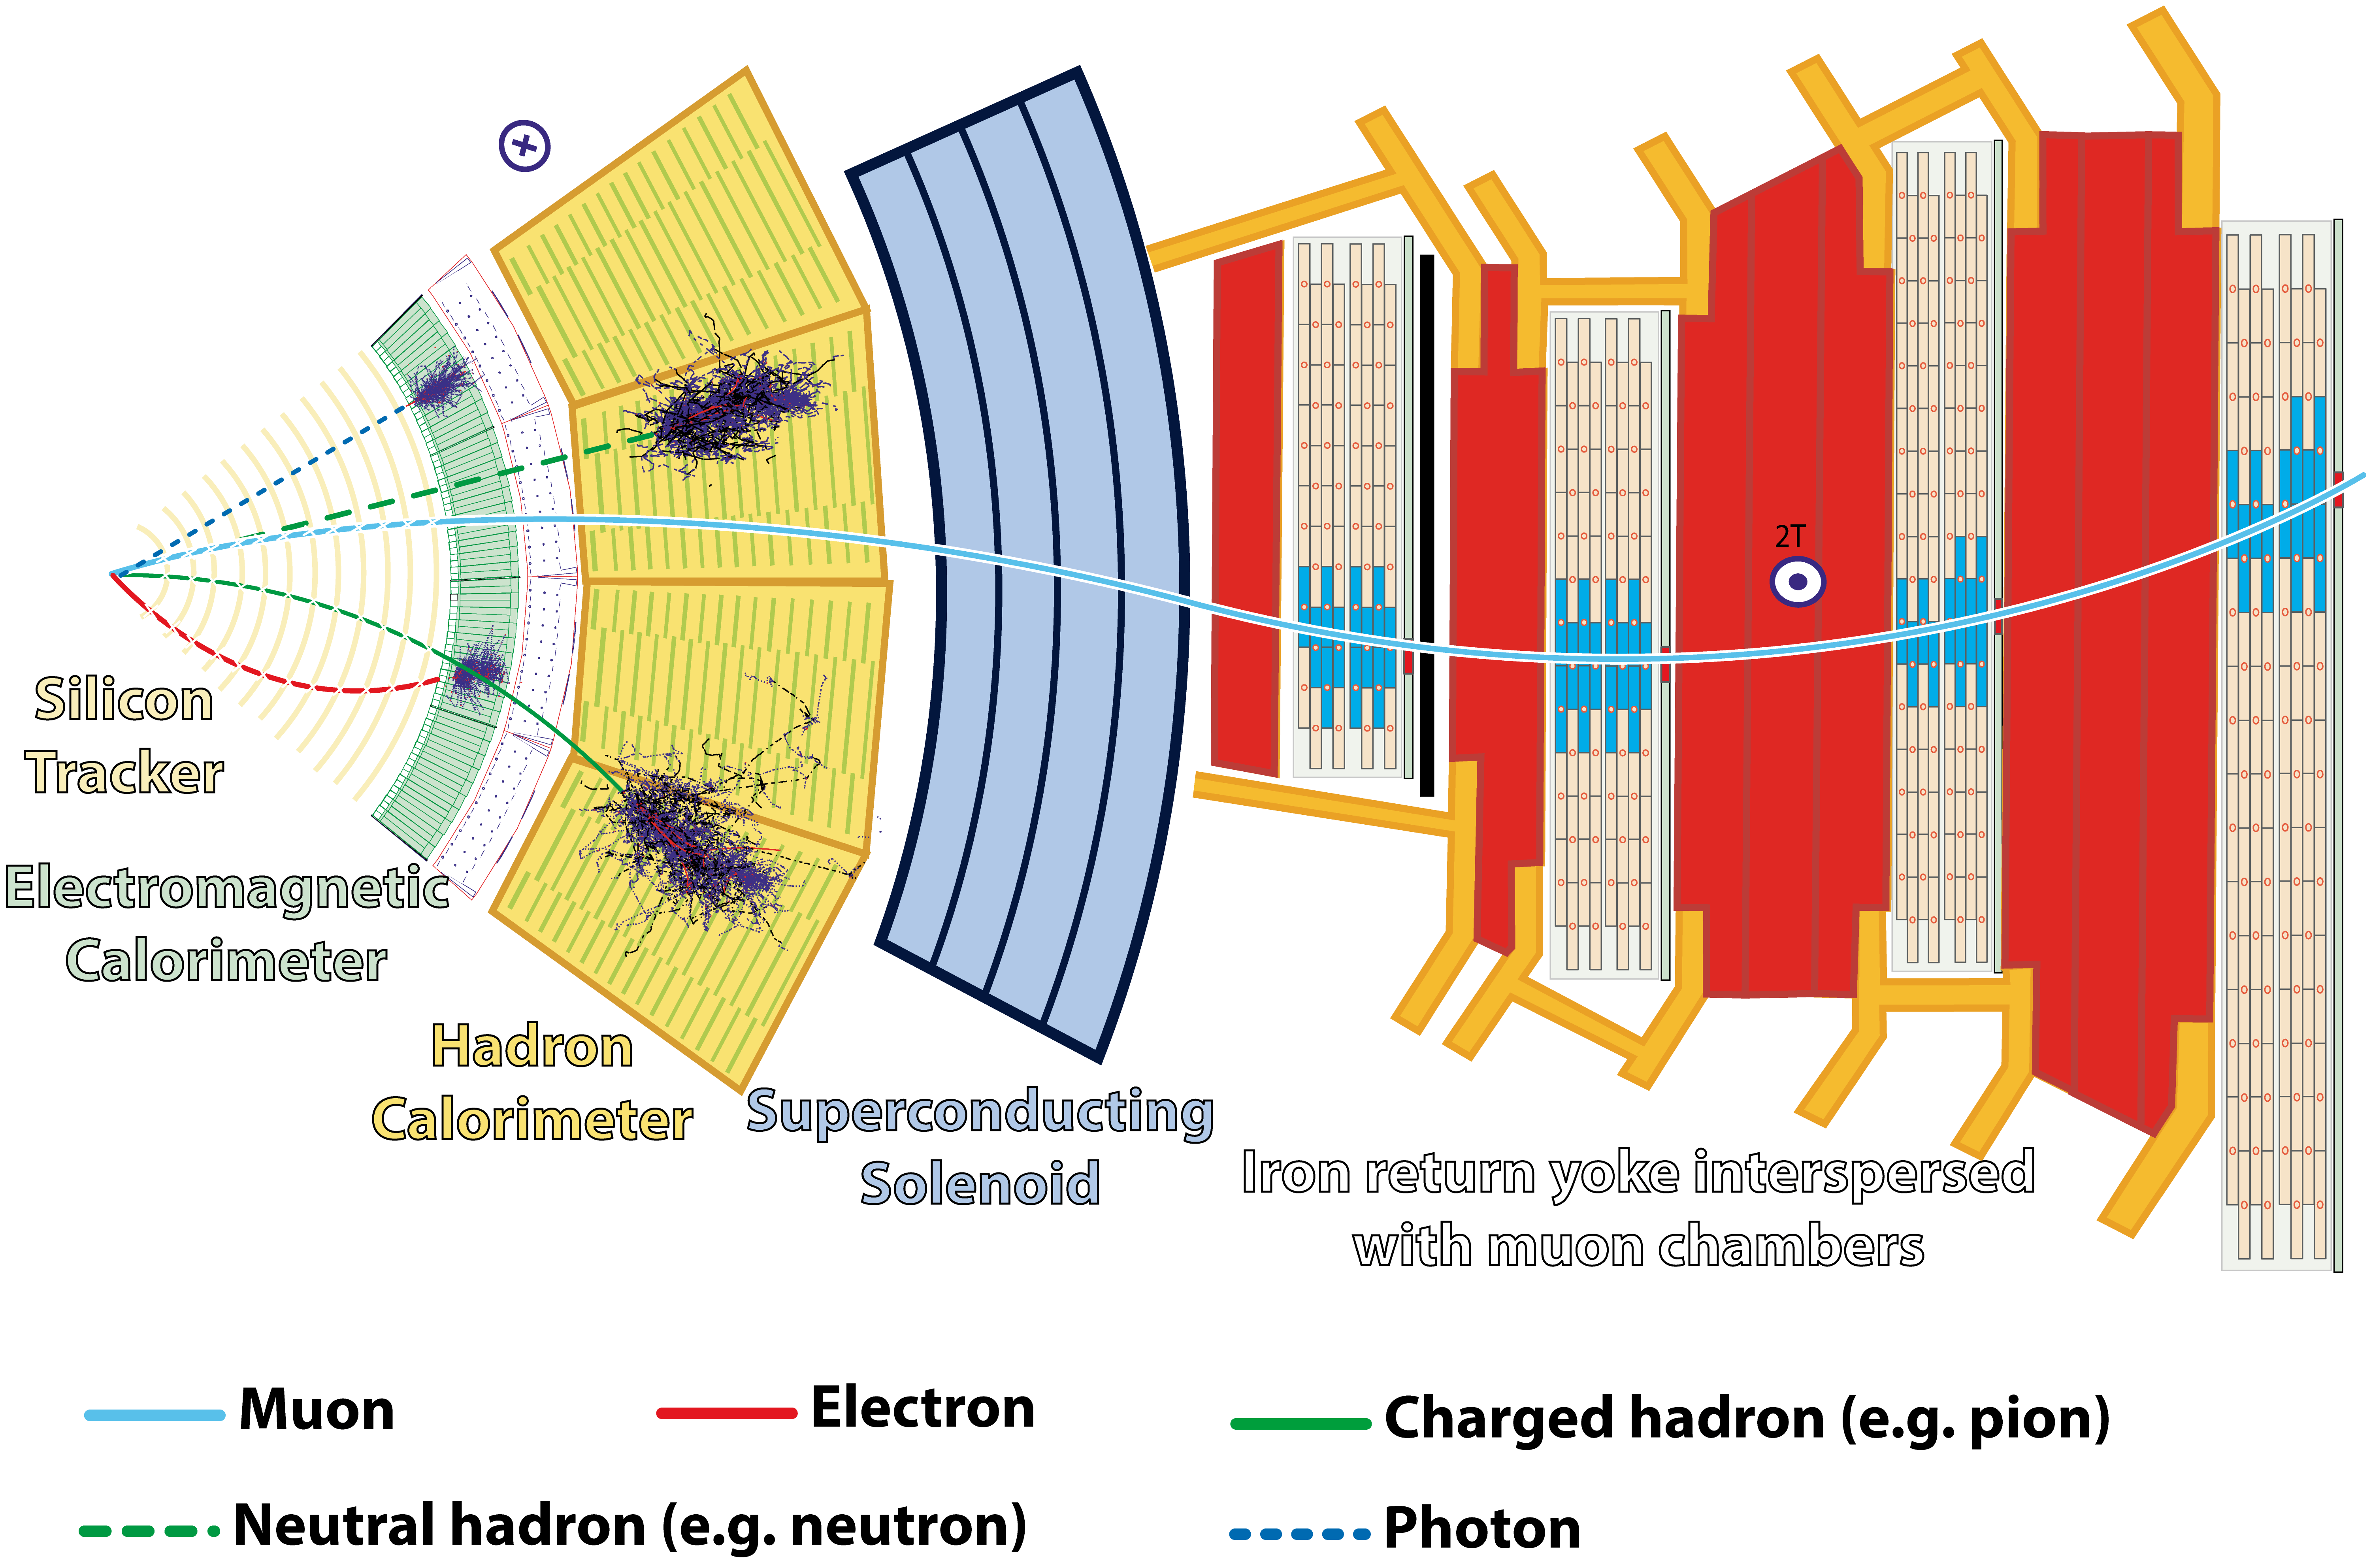
\includegraphics[width=0.8\textwidth]{images/cms_slide.png}
    \caption{Onion-like crossection of CMS. Image retrieved from \cite{cms_onion}}
    \label{fig:cms_slide}
\end{figure}


%%%%%%%%%%%%%%%%%%%%%%
%     CMS-DAQ
%%%%%%%%%%%%%%%%%%%%%%

\section{Data Acquisition (DAQ)}


According to \cite{cms_tridas_2002}, the collision rate takes around 40Mhz (100 Tbyte/s) which is impossible for the instrument to collect all of those signals that happen at a time.
The harvested signal that CMS detector select is determined from low-level trigger where the detector frontend (electronic circuit determination) process to select an interesting signal.
The level-1 (L1) trigger filter and produce the signal at 100 kHz (100 Gbyte/s). Then it has been sent to high-level trigger (HLT) where we could start to really see the interpretable physical quantities from here.

\subsection{CMS Online System}

CMS team also provide the tools for automate data acquisition as \cite{cms_daq} where the big picture has been demonstrated in Figure \ref{fig:cms_online_system}.
Apparently, the system still needs some people to double-check by using various tools e.g. Web GUI and so on during the running process of beam collider in LHC from the low-level system to high-level system.
\begin{figure}[h!]
    \centering
    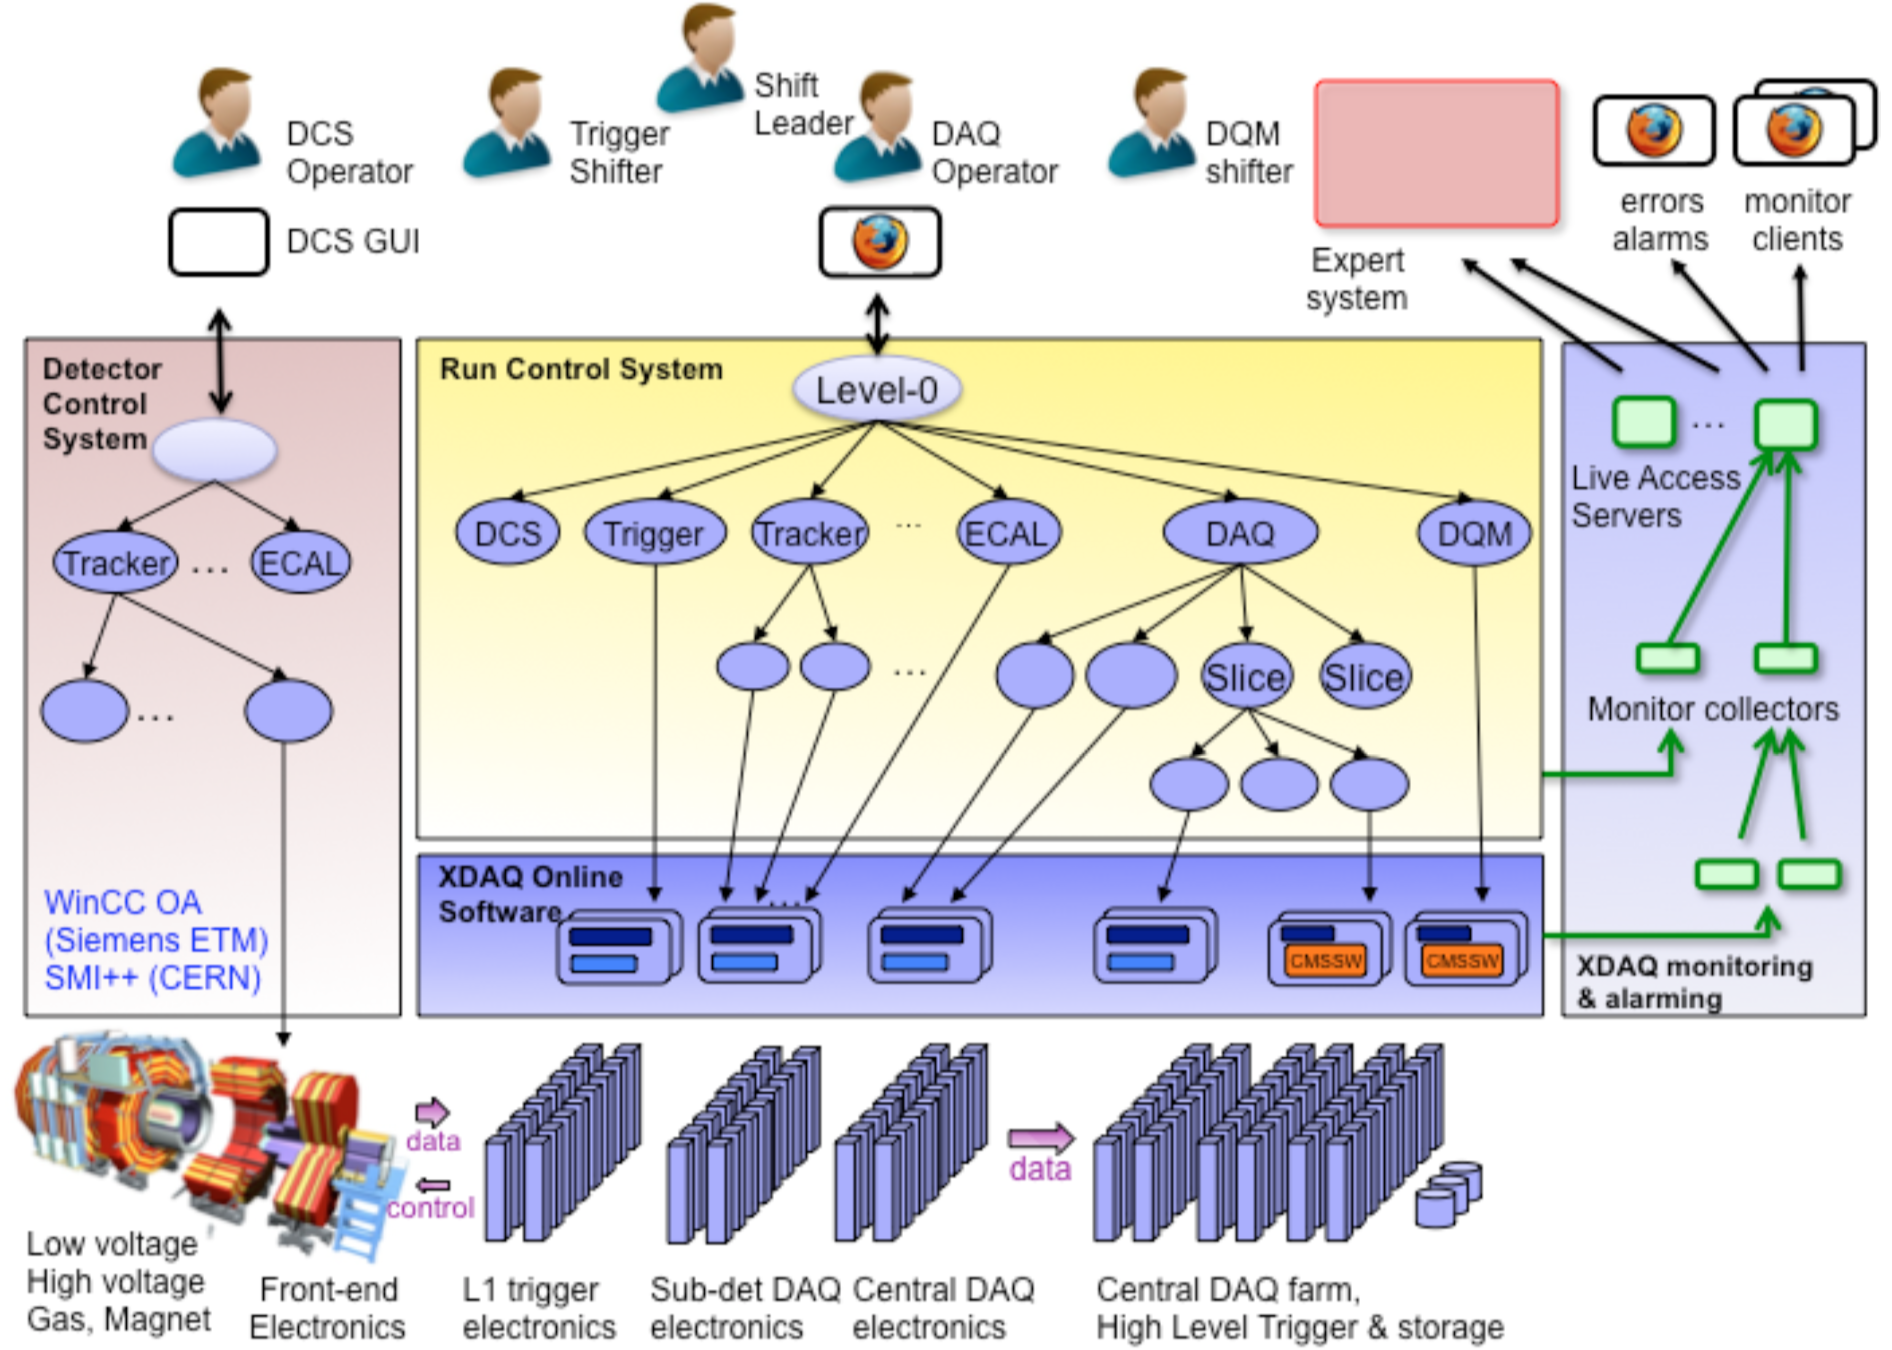
\includegraphics[width=\textwidth]{images/cms_online_system.png}
    \caption{Overview of the CMS online systems. Image retrieved from \cite{cms_daq}}
    \label{fig:cms_online_system}
\end{figure}

\subsection{Data Granularity}

We decide to divide a big chunk of data into one run and each run contains multiple lumisection which has 23 seconds of interval due to the beam does not change much where we consider 23 seconds of time.
Moreover, each lumisection contain multiple events. If we consider in terms of time to reconstruction, there are Express and PromptReco where data are reconstructed at nearly real-time and two days after a collision.

% \begin{table}[ht]
% \center
% \begin{tabular}{cc|c}
% A & B & A XOR B\\
% \hline
% 0 & 0 & 0\\
% 0 & 1 & 1\\
% 1 & 0 & 1\\
% 1 & 1 & 0\\
% \end{tabular}
% \caption{A simple table in \LaTeX.}
% \label{tab:xor}
% \end{table}


%%%%%%%%%%%%%%%%%%%%%%
%     CMS-DQM
%%%%%%%%%%%%%%%%%%%%%%

\section{Data Quality Monitoring (DQM)}

In order to make sure that data quality is nearly perfectly well collected, there is another story called DQM where it's actually the subset of the run control system in Figure \ref{fig:cms_online_system}.
CMS DQM team provides the tool where there is online and offline shifter checking the result from beam collision real-time and 48 hours after collision orderly. Figure \ref{fig:dqm_flow} is the schematic of a DQM workflow include the tools and person who responsible for each module.
If some sub-systems went weird such as the peak of the histogram drastically increase with no physical sense or some part of the detector turned off, they will report in the log of the system in the running process and calling detector experts to inspect the problem.
In this work, we will only focus on the red box which is the offline world.

\begin{figure}[h!]
    \centering
    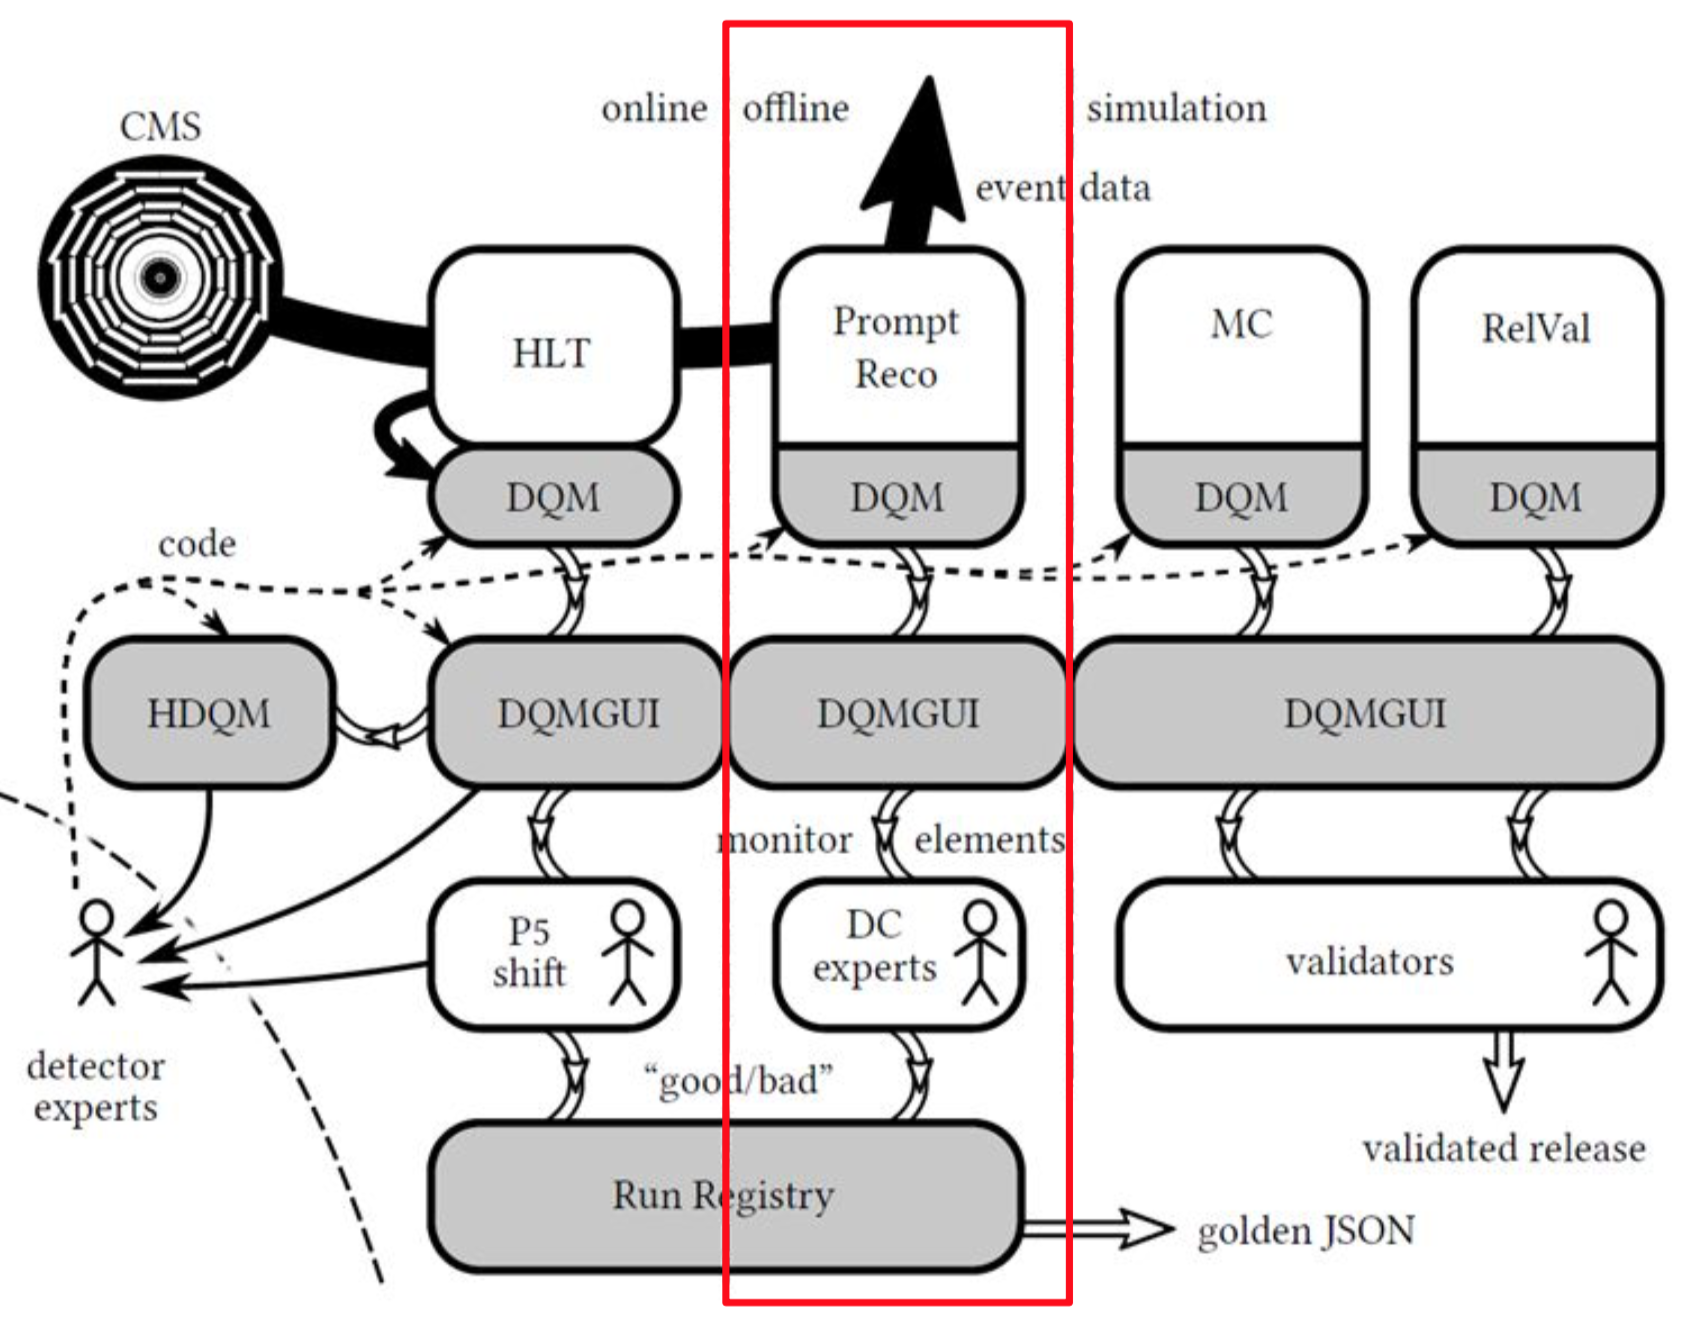
\includegraphics[width=0.7\textwidth]{images/dqm_flow.png}
    \caption{Tools and Processes of DQM. Image retrieved from M. Schneider, CHEP 2018}
    \label{fig:dqm_flow}
\end{figure}

Regarding the scope that we want to mimic, offline shifter and detector experts check a multiple distribution histogram to inspect and certify data quality.
The certification is made on run and lumisection granularity. The procedure to certify the data are the following list
\begin{enumerate}
    \item Automatically filter by DCS bits, beam status and etc. (LS levels)
    \item Runs tagged as bad by human (whole run)
    \item In rare cases are marked by DC experts (LS levels)
\end{enumerate}
Then the rest of them that pass all of those criteria are defined in Golden JSON which are good LS.
